%!TEX root = report.tex

\chapter{État de l'art}
\section{Introduction}

Dans ce chapitre on présente une étude du marché en énumérant les
applications dont les fonctionnalités sont équivalentes à la notre tout
en soulignant les différences qui subsistent. Ensuite on présente la
plate-forme ciblée et on passe en revu l’architecture d’une application
\android{}.

\section{Étude de marché}

Plusieurs sociétés offrent des solutions en relation avec celle proposée
par ce présent rapport. Malheureusement, la plupart d’entre elles sont
des solutions commerciales et, faute de documentation disponible, on n’a
pas pu les étudier d’un point de vu techno-technique et on s’est
contenté de relayer leurs caractéristiques tel que présenté dans les
sources citées.

\paragraph{NB:} % (fold) 
\label{par:nb}

Les solutions présentées ici sont le fruit des sociétés bien établies avec des ressources considérables et des salariés professionnels. Les comparer avec le travail incubé dans ce rapport serait abusif, l’indulgence est de mise.

\subsection{MIAA - Palomar Pomerado Health}

\begin{figure}
\centering
\subfloat{
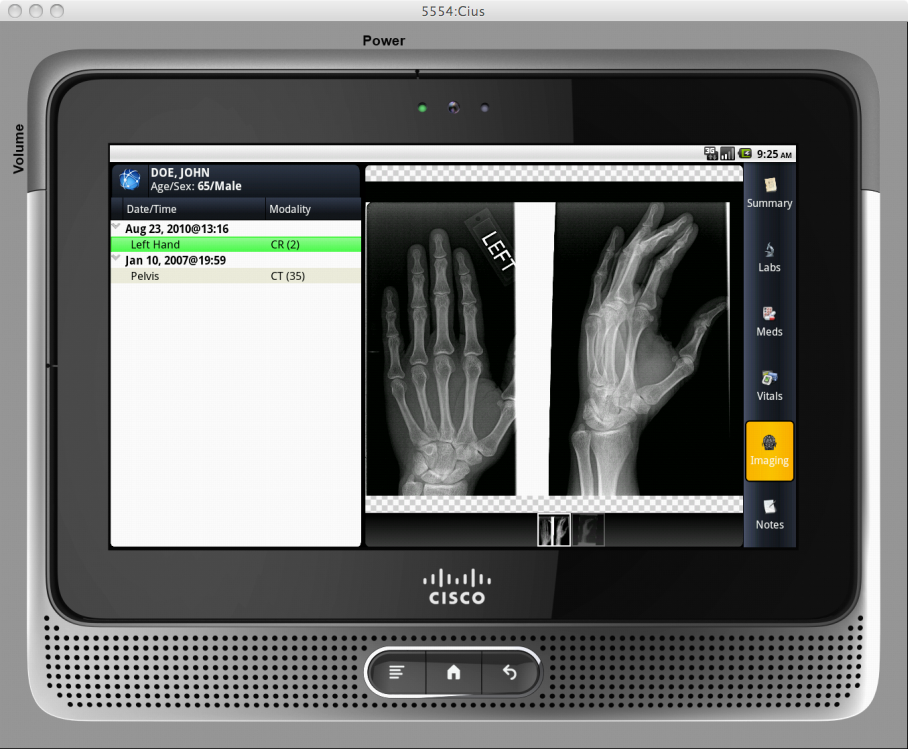
\includegraphics[width=0.5\textwidth]{pph1}
}\\
\subfloat{
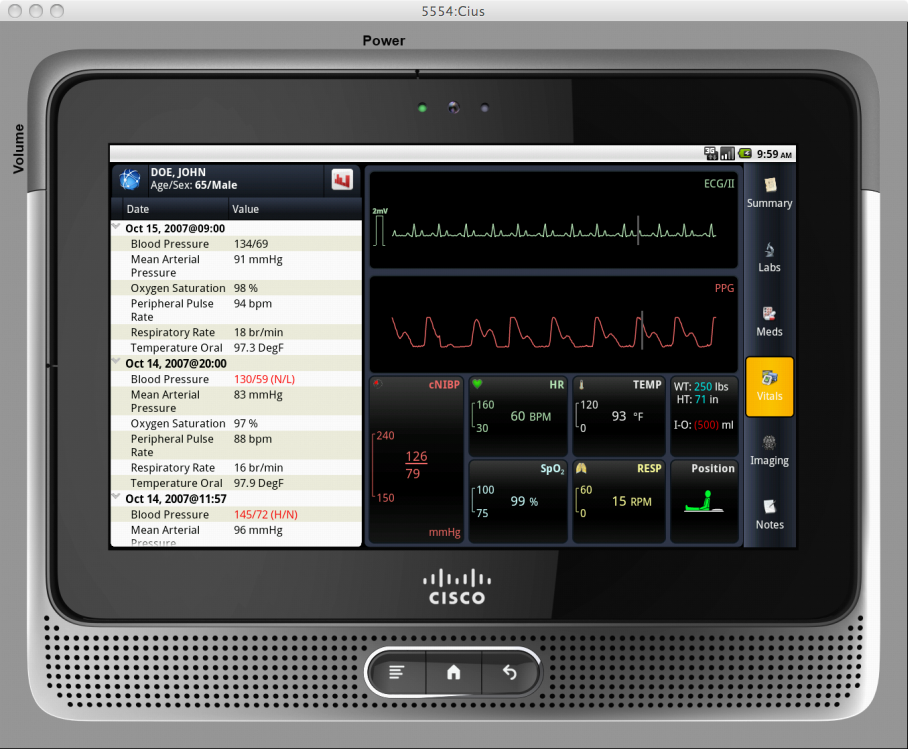
\includegraphics[width=0.5\textwidth]{pph2}
}\\
\subfloat{
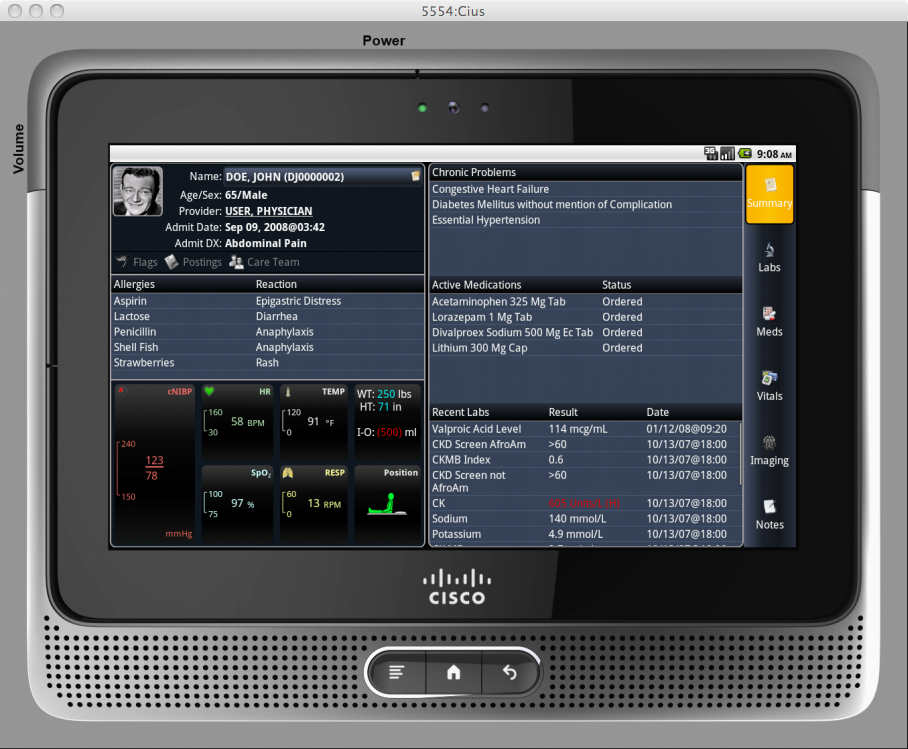
\includegraphics[width=0.5\textwidth]{pph3}
}
\caption{\gls{miaa} sur un émulateur Cisco Cius}
\label{fig:miaa}
\end{figure}

\gls{miaa} (figure \ref{fig:miaa}) est une application mobile issu d'un
projet R\&D chez \en{Palomar Pomerado Health}, l'institution publique la
plus large dans l'état de Californie (USA). Elle permet aux médecins
d'accéder rapidement au dossier médical complet du patient depuis une
variété de sources différentes qui s'affranchient des frontières des
organisations\cite{pph:eweek}. Elle vise les terminaux équipés avec le
système d'exploitation \android{} comme les smartphones et les
tablettes. \en{Palomar Pomerado Health} a choisi de déployer cette
application dans le \en{Palomar Medical Center} à \en{Escondido} (319
lits) et le \en{Pomerado Hospital} à \en{Poway} (107 lits) sur des
tablettes Cisco Cius\cite{pph:tabtimes}, ce choix s'est basé sur le
support qu'offre Cisco pour ces équipements.

Les avantages de \gls{miaa} sont:~\cite{pph:yahoo}

\begin{itemize}

\item Application mobile facile à utiliser conçue spécifiquement aux
médecins, tournant sur la plate-forme \android{}.

\item Un service \en{Cloud} qui fournit un accès permanent à
l'historique médical des patients à partir de divers sources de
données qui s'affranchient des frontières des organisations.

\item Interopérabilité avec les pionniers des systèmes électroniques
de l'historique médical tel que Cerner - \tm{Millennnium},
\tm{NextGen}, et \en{Veterans Administration} - \tm{VistA}.

\item Intégration en temps-réel des technologies de surveillance
des signes vitaux sans fils comme l'ECG, SPO$_{2}$, rythme cardiaque,
température, respiration, et pression du sang à partir des équipements
sans-fils.

\item Affichage des informations génétiques personnelles.

\item Application dynamique qui s’ajuste automatiquement à l’hôpital, clinique, et à la maison.

\item Simple, facile à utiliser, avec une tactile de nouvelle génération.

\item Intégration d’une messagerie inter-médecins sécurisée tout en maintenant le contexte du patient.

\item Des plan futurs pour intégrer NHIN \en{Connect} et les services
\en{Direct}.

\end{itemize}

\subsection{\pct{} - Cerner}

\begin{figure}[H]
\centering

\includegraphics[width=0.3\textwidth]{logo_cerner}
\end{figure}

\pct{} est une solution mobile conçue par le laboratoire Cerner qui
fait parti de l'ensemble de solutions \tm{Millennium+} et qui permet de
faciliter le travail des médecins. Elle offre une expérience native
sur iPad pour gérer les visites médicales et permet aux médecins
d'effectuer tout une visite typique qui inclue:~\cite{pct:flyer}

\begin{itemize}

\item Consultation des emplois du temps et les chartes des patients.

\item Satisfaire les demandes récurrentes comme les commandes simples
et les recharges des médicaments.

\item Consultation des diagnostics et résultats cliniques.

\item Documenter les allergies, les problèmes de santé et l'historique
du patient.

\item Créer et signer les notes de progressions.

\end{itemize}

Dès la fin du flux de travail du médecin ambulant. Cerner étend ces
mêmes fonctions et les adaptes aux établissements hospitaliers, les
urgences et les divers spécialistes.
Les avantages clés du \pct{} sont:~\cite{pct:flyer}

\begin{itemize}

\item Des réponses instantanées avec un flux de travail aisé.

\item Pas besoin de configurer l'application.

\item Adapter pour les visites médicales, aux patients et aux conditions
de la consultation.

\item Transmission sécurisée des données.

\item Des capacités de reconnaissance vocale.

\end{itemize}

\section{Le système d'exploitation \android{}}

\begin{figure}[H]
\begin{center}

\includegraphics[width=0.2\textwidth]{Android_robot.pdf}\\

\includegraphics[width=0.2\textwidth]{Android.pdf}
\end{center}
\caption{Logo et sigle d'\android{}}
\end{figure}

\android{} est un système d'exploitation basé sur Linux conçu pour les
équipements mobiles avec un écran tactile comme les \en{smartphones} et
les tablettes. Développé à l'origine par \en{\android{}, Inc.} que
\en{Google} a supporté financièrement et plus-tard acquis en 2005.
\android{} a été dévoilé en 2007 parallèlement à la fondation de
l'\en{Open Handset Alliance}: un consortium composé de sociétés dévoué à
l'avancement des standards ouverts pour les équipements mobiles. Le
premier téléphone  \android{} est sorti en Octobre 2008.

La dernière version stable d'\android{} en date (Mai 2013) est 4.2.2
\en{Jelly Bean} sortie le 11 Février 2013.

\android{} est basé sur le Kernel Linux et utilise pleinement ses capacités de supports matériels exhaustifs. Mais la comparaison avec les distributions Linux, embarqué ou même destiné aux bureaux, s'arrête à ce niveau.~\cite{lft:growth_android}

\begin{figure}
\centering
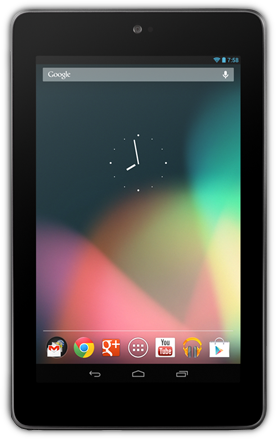
\includegraphics[width=0.4\textwidth]{nexus7}
\caption{\en{Google} Nexus 7, un terminal \android}
\end{figure}

\subsection{Parts du marché}

L’adoption du système d'exploitation \android{} suit une courbe
exponentielle depuis quelque temps et la tendance n'est pas prête de
s’inverser, selon le dernier rapport du cabinet d'analyse \en{Strategy
Analytics}, \android{} a réussi à capturer environ 68.4\% du marché
global \cite{venturebeat.com}.

\begin{table}[H]
\centering
\begin{tabular}{|m{0.2\textwidth}|m{0.13\textwidth}|m{0.13\textwidth}|m{0.13\textwidth}|m{0.13\textwidth}|m{0.13\textwidth}|}
\hline
\textsf{Système d'exploitation} &
\textsf{Volume de production 3Q2012\footnotemark[1]\footnotemark[3]} &
\textsf{Parts du Marché 3Q2012\footnotemark[1]} &
\textsf{Volume de production 3Q2011\footnotemark[2]\footnotemark[3]} &
\textsf{Parts du Marché 3Q2011\footnotemark[2]} & \textsf{Différence} \\ 
\hline
\android{} & 136.0 & 75.0\% & 71.0 & 57.5\% & 91.5\% \\
\hline
iOS & 26.9 & 14.9\% & 17.1 & 13.8\% & 57.3\% \\
\hline
BlackBerry & 7.7 & 4.3\% & 11.8 & 9.5\% & -34.7\% \\
\hline
Symbian & 4.1 & 2.3\% & 18.1 & 14.6\%  & -77.3\% \\
\hline
Windows Phone 7/ Windows Mobile & 3.6 & 2.0\% & 1.5 & 1.2\% & 140.0\% \\
\hline
Linux & 2.8 & 1.5\% & 4.1 & 3.3\% & -31.7\% \\
\hline
Autres & 0.0 & 0.0\% & 0.1 & 0.1\% & -100.0\% \\
\hline
\hline
Totales & 181.1 & 100.0\% & 123.7 & 100.0\% & 46.4\% \\ \hline
\end{tabular}

\caption{Les six major systèmes d'exploitation mobile en termes de Volume
et de parts de marché en 3\ieme trimestre 2012~\cite{idc}}

\label{tab:marketshareall}
\end{table}

\footnotetext[1]{3\ieme trimestre 2012}
\footnotetext[2]{3\ieme trimestre 2011}
\footnotetext[3]{En million d'unité}

\begin{table}[H]
\centering
\begin{tabular}{|m{0.3\textwidth}|m{0.1\textwidth}|m{0.1\textwidth}|m{0.1\textwidth}|m{0.1\textwidth}|m{0.1\textwidth}|}
\hline
& \textsf{2008} & \textsf{2009} & \textsf{2010} & \textsf{2011} &
\textsf{2012}\footnotemark[4]\\
\hline
\textsf{Unités \android{} produites} & 0.7 & 7.0 & 71.1 & 243.4 & 333.6\\
\hline
\textsf{Parts de marché \android{}} & 0.5\% & 4.0\% & 23.3\% & 49.2\%
& 68.2\%\\
\hline
\end{tabular}
\caption{Production et parts de marché entre 2008 et 2012~\cite{idc}}
\label{tab:marketshare}
\end{table}

\footnotetext[4]{Estimation}

\subsection{Versions \android{} en circulation}

Le tableau \ref{tab:androidversion} représente les différentes versions
d'\android{} et leurs taux d'utilisation respectifs. On remarque que
la plupart des terminaux mobiles \android{} sont sous la version 2.3
\en{Gingerbread} sortie le 6 Décembre 2010, Ceci est du aux fait que
plusieurs téléphones bas de gamme sont équipés de cette version et sont encore en production.

\begin{table}[H]
\centering
\begin{tabular}{|c|l|c|c|}
\hline
\textsf{Version} & \textsf{Codename} & \textsf{API} &
\textsf{Distribution}\\
\hline
1.6 & Donut & 4 & 0.2\%\\
\hline
2.1 & Eclair & 7 & 2.2\%\\
\hline
2.2 & Froyo & 8 & 8.1\%\\
\hline
2.3 - 2.3.2 & Gingerbread & 9 & 0.2\% \\
\cline{1-1}\cline{3-4}
2.3.3 - 2.3.7 & & 10 & 45.4\%\\
\hline
3.1 & Honeycomb & 12 & 0.3\%\\
\cline{1-1}\cline{3-4}
3.2 & & 13 & 1.0\%\\
\hline
4.0.3 - 4.0.4 & Ice Cream Sandwich & 15 & 29.0\%\\
\hline
4.1 & Jelly Bean & 16 & 12.2\%\\
\cline{1-1}\cline{3-4}
4.2 & & 17 & 1.4\%\\
\hline
\end{tabular}
\caption{Distribution des versions \android{} en circulation qui ont
accédé au \en{Google Play}\protect\footnotemark[5]}
\label{tab:androidversion}
\end{table}

\footnotetext[5]{Données récoltées pendant une période de tests de 14
jours arrêtée le 4 Février 2013.}
%%%ENDsubsection

\subsection[Les raisons du succès d'\android{}]{Les raisons du succès d'\android{}\cite{lft:growth_android}}

Les raisons pour le succès \android{} peuvent être
dénombrées comme suit:

\begin{description}

\item [Un \en{Framework} d'Application Riche.] \android{} fournit un
excellent \gls{sdk} avec des \gls{api} stable à long-terme, ce qui
assure aux partenaires tiers un écosystème standardisé. Alors que le
système en lui même est en constante évolution, la stabilité des
\gls{api} pour la plupart est préservée, ce qui permet d'investir dans
le long-terme. Concevoir et construire des applications pour les
distribuer sur différentes plate-formes permet des réductions drastiques en
termes des coûts et effort pour les entreprises.

\item [Un \gls{ttm} Agressif.] Concevoir des appareils avec \android{}
peut réduire le \gls{ttm} d'une manière significative. Il suffit de se
procurer les sources, les adapter pour le matériel en question et vendre. Et dans le cas ou les schémas et usages de référence sont
appliqués, la sortie d'un nouveau produit est possible au cours de quelque
mois. Seulement voilà, ce n'est pas aussi facile et une certaines expertises
et connaissances dans ce domaine sont requises. Et même si sortir un
système basé sur \android{} peut être plus rapide comparé à d'autres
solutions, le suivi des évolutions du système ainsi que maintenir le
code à long terme est une autre histoire.

\item [Concentrer sur \og Ce qui compte réellement \fg.] En fournissant
un \en{Framework} pratique, \android{} permet aux développeurs de se
concentrer sur les aspects à valeur commerciale. L'assemblage d'un
appareil est une activité qui consomme énormément de temps et de
ressources et n'a pas à réinventer un - encore - autre système d'exploitation permettant d'éviter un autre gaspillage de temps.

\item [Open Source.] Bien qu'il ne soit pas développé d'une manière
communautaire, \android{} reste 100\% modifiable et diffuse un sentiment
de sécurité parmi les entreprises contre les menaces légales.

\end{description}

\subsection[La pile logicielle d'\android{}]{La pile logicielle d'\android{}\cite{pa4ad:chptr1}}

D'une manière simple. La pile logicielle d'\android{} est un Kernel Linux et une collection de bibliothèques C/C++ exposée à travers un framework d'application qui fournit des services pour l'environnement d'exécution et les applications. On peut énumérer les éléments composant la pile logicielle comme suit:

\begin{description}

\item [Kernel Linux:]
Services de base qui incluent les pilotes matériels, gestion des processus et de la mémoire, sécurité, réseaux et gestion d'autonomie; fourni aussi une couche d'abstraction entre le matériel et le reste de la pile.

\item [Bibliothèque:]
Se situe au dessus du Kernel, \android{} inclue divers bibliothèques C/C++ de base comme \dev{libc} et \dev{SSL} ainsi que:

\begin{itemize}

\item Une bibliothèque multimédia pour la lecture des fichiers audio et vidéo.

\item Un \en{Surface manager} pour la gestion de l'affichage.

\item Des bibliothèques graphiques qui incluent le \dev{SGL} et \dev{OpenGL} pour les graphiques 2D et 3D.

\item Un support natif de base de données à travers la base de données \dev{SQLite}.

\item \dev{SSL} et \dev{WebKit} pour le navigateur web intégré et la sécurité internet.

\end{itemize}

\item [Environnement d'Execution (runtime) \android{}:]

L'environnement d’exécution et le facteur qui sépare un terminal \android{}
d'une implémentation Linux mobile. En cohérence avec les bibliothèques de base
et la machine virtuelle \dev{Dalvik}, l'environnement d’exécution \android{} est
le moteur qui fait fonctionner les applications et, avec les bibliothèques,
forme les bases du framework application.

\begin{description}

\item [Bibliothèque de Base:]

Même si la plus part des applications \android{} sont écrits avec du langage
\dev{Java}, \dev{Dalvik} n'est pas une machine virtuelle java. Les bibliothèques
\android{} de base fournit la plus part des fonctionnalités qu'on retrouve
dans les bibliothèques de base \dev{Java}, en plus de quelque bibliothèques
spécifiques à \android{}.

\item [La Machine Virtuelle dev{Dalvik}:]

\dev{Dalvik} est une machine virtuelle qui a était optimisée pour
s'assurer que chaque terminal peut faire fonctionner plusieurs instance
d'une manière efficace. Il s’appuie sur le Kernel Linux pour le
threading et la gestion bas niveaux de la mémoire.

\end{description}

\item [Le \en{Framework} Application:]

Le \en{Framework} application fournit les classes utilisées pour créer les application \android{}. Il fournit une abstraction générique pour l’accès matériel et gère l'\gls{ui} et les ressources de l'application.

\item [Couche Application:]

Toute application, quelle soit native ou produite par un tiers, est
construite sur la couche application via les même \gls{api}. La couche
application opère à l'intérieur de l'environnement d’exécution \android{},
utilisant les classes et les services mis à disposition par le \en{framework}
application.

\end{description}

\subsection[Architecture des applications \android{}]{Architecture des applications \android{}\cite{pa4ad:chptr1}}

L'architecture d'\android{} encourage la réutilisation des composants,
ce qui nous permet de publier et de partager des \en{Activities},
services, et données avec d'autres applications. Avec une gestion
d'accès gérée par les restrictions de sécurité que nous définissons.

Le même mécanisme qui nous permet de produire un gestionnaire de contact alternatif ou un compositeur de numéros nous permet aussi d'exposer les composants de notre application pour permettre à d'autres développeurs de les réutiliser en créant des nouveaux \gls{ui} ou d’étendre des fonctionnalités.

Les services application suivants représentent les bases architecturales de toute application \android{}, fournissant le \en{Framework} qu'on va utiliser pour notre application.

\begin{description}

\item [L'\dev{Activity Manager} et le \dev{Fragment Manager}:]
Contrôle le cycle de vie de nos \en{Activities} et nos \en{Fragments} respectivement, y inclue la gestion de la pile des \en{Activities}.

\item[\dev{Views}]
Utilisé pour construire l'\gls{ui} de notre \dev{Activities} et \dev{Fragments}.

\item[\dev{Notification Manager}:]
Fournit un mécanisme consistant et non-intrusif de signalisation pour l'utilisateur.

\item[\dev{Content Providers}:]
Permet à notre application le partage des données.

\item[\dev{Resource Manager}:]
Offre un moyen d'externaliser les ressources (comme par exemple les chaînes de caractères et les images.)

\item[\dev{Intents}:]
Présente un mécanisme pour transférer les données entre les applications et leurs composants.

\end{description}

Parmi les fonctionnalités les plus intéressantes pour l'aboutissement de notre projet offerte par \android{} sont ses capacités de localisation, étudiées dans la partie suivante.

\subsection{Location Based Services}

\subsubsection{Concept}

Pour positionner un terminal, on spécifie ses coordonnées géographiques
en utilisant le géo-codage.

\paragraph[Géo-codage]{Géo-codage\cite{wiki:geocoding}}

Le géo-codage est le processus de retrouver les coordonnées
géographiques associées (exprimées souvent en terme de \textit{latitude}
et \textit{longitude}) d'après d'autre données géographiques comme
l'adresse de la rue, code postal. Ces coordonnées géographiques peuvent
être insérées dans un système d'informations géographiques ou intégrés dans
des médias comme les photos numériques par le biais de géo-marquage.
Cette opération est communément appelée le \en{Forward Geocoding}.

Le \en{Reverse Geocoding} est la procédure inverse: retrouver les lieux textuel comme l'adresse de la rue d'après les coordonnés géographiques. Car même si l'usage des paramètres comme la longitude et la latitude fournit un moyen pratique pour localiser l'individu d'une manière relativement précise. Les utilisateurs penchent à penser en terme de rues et adresses.

A fin de déterminer la position du terminal, plusieurs technologie de localisation sont à notre disposition.

\paragraph[Localisation par GSM]{Localisation par GSM}

On peut retrouver la position du terminal mobile par le biais de sa
cellule \gls{gsm}. Cette technique fait intervenir divers moyens de
triangulation des signaux parvenant depuis les cellules qui desservent
un téléphone mobile. La position géographique du terminal est déterminée
par une multitude de méthodes comme la \gls{tdoa} ou l'\gls{e-otd}.

\paragraph[Localisation parGPS]{Localisation parGPS\cite{enig:gps}}

\gls{gps} est un système de navigation par satellites qui fourni la
localisation et le temps dans toute condition météorologique et partout
sur terre s'il existe un accès non bloquant à 4 satellites
\gls{gps} ou plus. Ce Système fournit des services essentiels dans le domaine
militaire, civil et commercial partout dans le monde. Il est maintenu
par les États Unis d'Amérique et accessible à quiconque possédant un
récepteur \gls{gps}.

\subsubsection[La localisation dans \android{}]{La localisation dans \android{}\cite{pa4ad:chptr13}}\label{sss:android_localisation}

L'accès aux \gls{lbs} se fait essentiellement via deux objets:
\begin{description}
\item [\dev{Location Manager}]\footnote{android.location.LocationManager} Permet d'exploiter les services basés sur la localisation.
\item [\dev{Location Providers}]\footnote{android.location.LocationProvider} Chaque \en{Providers} représente une technologie de localisation utilisé afin de déterminer la localisation actuelle du terminal.

\end{description}
On utilise ces deux Classes pour les fins suivantes:
\begin{itemize}
\item Obtenir la position actuelle.
\item Suivre les mouvements.
\item Alerte de proximité dans le cas ou l'on approche ou l'on s’éloigne d'une zone spécifique.
\item Retrouver les fournisseurs de localisation disponible.
\item Observer le status du récepteur \gls{gps}.
\end{itemize}

Généralement deux techniques de détection de localisation sont disponibles dans le terminal: détection par le réseau \en{Network Provider} et la détection par \gls{gps} (\en{GPS Provider}). Le choix de la technologie à utiliser est soit explicite ou automatique suivant des critères prédéfinis par le développeur de l'application. Avant de pouvoir exploiter un service de localisation, un niveau de précision doit figurer dans le manifeste de l'application via les \dev{uses-permission} \en{tags}.

\paragraph{Niveau de permission \textbf{COARSE} } % (fold)
\label{par:coarse}

\begin{lstlisting}[language=xml, caption=Permission pour la localisation par le réseau.]
<uses-permission android:name="android.permission.ACCESS_COARSE_LOCATION"/>
\end{lstlisting}
% paragraph par:coarse (end)

\paragraph{niveau de permission \textbf{FINE} } % (fold)
\label{par:fine}

\begin{lstlisting}[language=xml, caption=Permission pour la localisation par GPS.]
<uses-permission android:name="android.permission.ACCESS_FINE_LOCATION"/>
\end{lstlisting}

A noter qu'une application ayant la permission \dev{FINE} possède implicitement la permission \dev{COARSE}.

Avoir la localisation dans la plate-forme \android{} se fait par le biais de
\en{callback}, on indique au \dev{LocationManager} qu'on veut recevoir des mises
à jour de la localisation par la fonction \dev{requestLocationUpdates()} en lui
passant une implémentation de
\dev{LocationListener}\footnote{android.location.LocationListener}. Cette
interface contient plusieurs fonctions de \en{callback} que le
\dev{LocationManager} appelle quand la localisation de l'utilisateur change ou
l'état du service change\cite{guide:location_strategies}.
